\documentclass{article}

\setlength{\headsep}{0.75 in}
\setlength{\parindent}{0 in}
\setlength{\parskip}{0.1 in}

%=====================================================
% Add PACKAGES Here (You typically would not need to):
%=====================================================

\usepackage{xcolor}
\usepackage[margin=1in]{geometry}
\usepackage{amsmath,amsthm}
\usepackage{fancyhdr}
\usepackage{enumitem}
\usepackage{graphicx}
\usepackage{amsmath, amssymb}  % Include the amsmath and amssymb packages for mathematical symbols

%=====================================================
% Ignore This Part (But Do NOT Delete It:)
%=====================================================

\theoremstyle{definition}
\newtheorem{problem}{Problem}
\newtheorem*{fun}{Fun with Algorithms}
\newtheorem*{challenge}{Challenge Yourself}
\def\fline{\rule{0.75\linewidth}{0.5pt}}
\newcommand{\finishline}{\begin{center}\fline\end{center}}
\newtheorem*{solution*}{Solution}
\newenvironment{solution}{\begin{solution*}}{{\finishline} \end{solution*}}
\newcommand{\grade}[1]{\hfill{\textbf{($\mathbf{#1}$ points)}}}
\newcommand{\thisdate}{March 7, 2024}
\newcommand{\thissemester}{\textbf{Rutgers: Spring 2024}}
\newcommand{\thiscourse}{ECE 509: Convex Optimization} 
\newcommand{\thishomework}{Number} 
\newcommand{\thisname}{Name} 
\newcommand{\thisextension}{Yes/No} 

\headheight 40pt              
\headsep 10pt
\renewcommand{\headrulewidth}{0pt}
\pagestyle{fancy}

\newcommand{\thisheading}{
   \noindent
   \begin{center}
   \framebox{
      \vbox{\vspace{2mm}
    \hbox to 6.28in { \textbf{\thiscourse \hfill \thissemester} }
       \vspace{4mm}
       \hbox to 6.28in { {\Large \hfill Homework \#\thishomework \hfill} }
       \vspace{2mm}
         \hbox to 6.28in { { \hfill \thisdate  \hfill} }
       \vspace{2mm}
       \hbox to 6.28in { \emph{Name: \thisname \hfill Extension: \thisextension}}
      \vspace{2mm}}
      }
   \end{center}
   \bigskip
}

%=====================================================
% Some useful MACROS (you can define your own in the same exact way also)
%=====================================================


\newcommand{\ceil}[1]{{\left\lceil{#1}\right\rceil}}
\newcommand{\floor}[1]{{\left\lfloor{#1}\right\rfloor}}
\newcommand{\prob}[1]{\Pr\paren{#1}}
\newcommand{\expect}[1]{\Exp\bracket{#1}}
\newcommand{\var}[1]{\textnormal{Var}\bracket{#1}}
\newcommand{\set}[1]{\ensuremath{\left\{ #1 \right\}}}
\newcommand{\poly}{\mbox{\rm poly}}


%=====================================================
% Fill Out This Part With Your Own Information:
%=====================================================


\renewcommand{\thishomework}{5} %Homework number
\renewcommand{\thisname}{Ravi Raghavan} % Enter your name here
\renewcommand{\thisextension}{No} % Pick only one of the two options accordingly

\begin{document}

\thisheading
\vspace{-0.75cm}


%=====================================================
% LaTeX Tip: You can erase this part from here.... 
%=====================================================		

\finishline

%=====================================================
% LaTeX Tip: ... to here
%=====================================================	


\bigskip

\begin{problem} \textit{Steepest descent method in $l_{\infty}$-norm.} Explain how to find a steepest descent direction in the $l_{\infty}$-norm, and give a simple interpretation.

\begin{solution}
    $\Delta x_{sd} = ||\nabla f(x)||_* \Delta x_{nsd}$ \newline 
    $x_{nsd} = \arg \min_{x} \{\nabla f(x)^T x \enspace | \enspace ||x||_{\infty} \leq 1 \}$ \newline 
    $||\nabla f(x)||_* = sup \{\nabla f(x)^T x \enspace | \enspace ||x||_{\infty} \leq 1\}$ \newline 

    We know that the dual norm of the $l_{\infty}$-norm is just the $l_{1}$-norm. Hence, we can say that $||\nabla f(x)||_*$, under the $l_{\infty}$-norm, is just $||\nabla f(x)||_1$

    When analyzing the normalized steepest descent direction, it is clear to see that $x_{nsd} = -sign(\nabla f(x))$. To clarify, the $sign$ function is applied component-wise to $\nabla f(x)$ 

    Hence, the unnormalized steepest descent direction is just $\Delta x_{sd} = -||\nabla f(x)||_1 sign(\nabla f(x))$ \newline


    \textbf{\underline{Simple Interpretation:}} If the partial derivative of the function $f$ with respect to $x_i$ is positive, we will have to reduce $x_i$. This makes sense because it will be like reducing $f$ as well. On the other hand, if the partial derivative of the function $f$ with respect to $x_i$ is negative, we will increase $x_i$. This makes sense because it will be like reducing $f$ as well. 
    
\end{solution}

\end{problem}

\begin{problem} \textit{The pure Newton method.} Newton’s method with fixed step size $t = 1$ can diverge if the initial point is not close to $x^*$. In this problem we consider two examples. 
\begin{enumerate}
    \item[(a)] $f(x) = \log{(e^x + e^{-x})}$ has a unique minimizer $x^* = 0$. Run Newton’s method with fixed step size $t = 1$, starting at $x^{(0)} = 1$ and at $x^{(0)} = 1.1$
    \begin{solution} $x^{*} = 0$, $p^{*} = f(x^{*}) = 0.6931471805599453$

    $\nabla(f(x)) = \frac{e^x - e^{-x}}{e^x + e^{-x}}$ \newline 
    $\nabla^2(f(x)) = \frac{(e^x + e^{-x})^2 - (e^x - e^{-x})^2}{(e^x + e^{-x})^2} = \frac{4}{(e^x + e^{-x})^2}$

    $x^{(0)} = 1$ \newline 
    $\Delta x_{nt} = -\frac{\nabla(f(x))}{\nabla^2(f(x))} = h(x)$ \newline 

    $h(0) = -\frac{\nabla(f(x^{(0)}))}{\nabla^2(f(x^{(0)}))} = - \frac{0.761594155956}{0.419974341614} = -1.81343020392$ \newline 

    $x^{(1)} = x^{(0)} + h(x^{(0})) = 1 - 1.81343020392 = -0.813430203924 = -8.134 \cdot 10^{-1}$

    $x^{(2)} = x^{(1)} + h(x^{(1})) = -0.813430203924 + 1.22283252051 = 0.409402316586 = 4.094 \cdot 10^{-1}$

    $x^{(3)} = x^{(2)} + h(x^{(2})) = 0.409402316586 - 0.456707233043 = - 0.047304916457 = -4.730 \cdot 10^{-2}$

    $x^{(4)} = x^{(3)} + h(x^{(3})) = -0.047304916457 + 0.0473755192607 = 0.0000706028 = 7.060 \cdot 10^{-5}$
    
    $x^{(5)} = x^{(4)} + h(x^{(4})) = 0.0000706028 - 0.0000706028039346 = -2.347 \cdot 10^{-13}$

    \begin{table}[h]
    \centering
    \begin{tabular}{|c|c|c|c|}
        \hline
        k & $x^{(k)}$ & $f(x^{(k)})$ & $f(x^{(k)}) - p^*$ \\
        \hline
        0 & $1$ & 1.1269280110429725 & 0.4337808304830272 \\
        1 & $-8.134 \cdot 10^{-1}$ & 0.9928690093583381 & 0.2997218287983928 \\
        2 & $4.094 \cdot 10^{-1}$ & 0.7747107967452456 & 0.08156361618530028\\
        3 & $-4.730 \cdot 10^{-2}$ & 0.6942656410735625 & 0.0011184605136171921\\
        4 & $7.060 \cdot 10^{-5}$ & 0.6931471830523231 & $2.4923778597 \cdot 10^{-9}$\\
        5 & $-2.347 \cdot 10^{-13}$ & 0.6931471805599453 & $5.4733995 \cdot 10^{-14}$\\
        \hline
    \end{tabular}
    \caption{Newton's Method: $x^{(0)} = 1$}
    \label{tab:mytable}
\end{table}


Now, let's change $x^{(0)} = 1.1$ 

$x^{(1)} = x^{(0)} + h(x^{(0})) = - 1.12855258527$

    $x^{(2)} = x^{(1)} + h(x^{(1})) = 1.23413113304$

    $x^{(3)} = x^{(2)} + h(x^{(2})) = - 1.69516597992$

    $x^{(4)} = x^{(3)} + h(x^{(3})) = 5.71536010038$
    
    $x^{(5)} = x^{(4)} + h(x^{(4})) = - 23021.3564857$

    \begin{table}[h]
    \centering
    \begin{tabular}{|c|c|c|c|}
        \hline
        k & $x^{(k)}$ & $f(x^{(k)})$ & $f(x^{(k)}) - p^*$ \\
        \hline
        0 & $1.1$ & 1.205083319768696 & 0.5119361392087508 \\
        1 & $- 1.12855258527$ & 1.22808384311 & 0.534936662546 \\
        2 & $1.23413113304$ & 1.31546405981 & 0.622316879246\\
        3 & $- 1.69516597992$ & 1.72830814921 & 1.03516096865\\
        4 & $5.71536010038$ & 5.71537095711 & $5.02222377655$\\
        5 & $- 23021.3564857$ & $23021.3564857$ & $23020.6633385$\\
        \hline
    \end{tabular}
    \caption{Newton's Method: $x^{(0)} = 1$}
    \label{tab:mytable}
\end{table}

\begin{figure}[h!]
        \centering
        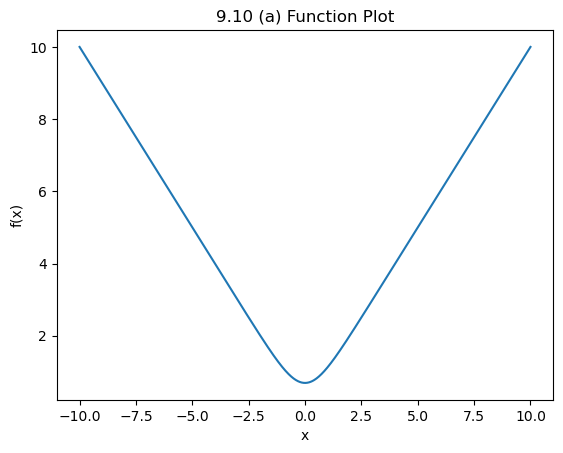
\includegraphics[width=0.7\textwidth]{HW5-9-10(a).png}
        \caption{Plot of $f(x)$}
    \end{figure}  

\begin{figure}[h!]
        \centering
        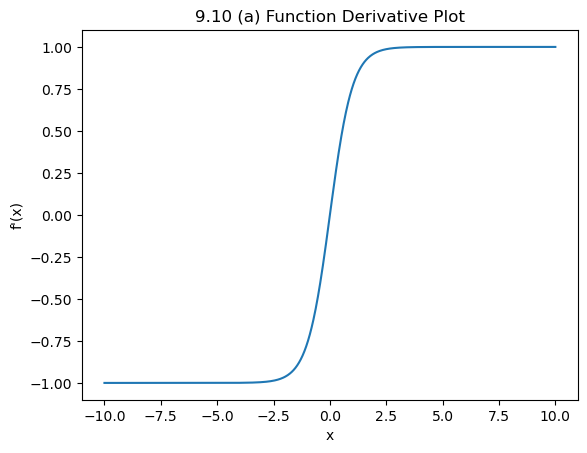
\includegraphics[width=0.7\textwidth]{HW5-9-10(a)-Derivative.png}
        \caption{Plot of $f^{'}(x)$}
    \end{figure}  
        
    \end{solution}
\newpage 
    \item[(b)] $f(x) = -\log{(x)} + x$ has a unique minimizer $x^* = 1$. Run Newton’s method with fixed step size $t = 1$, starting at $x^{(0)} = 3$

    \begin{solution}
        $\nabla(f(x)) = \frac{-1}{x} + 1 = \frac{x - 1}{x}$ \newline 
    $\nabla^2(f(x)) = \frac{1}{x^2}$

    $\Delta x_{nt} = h(x) = -\frac{\nabla(f(x))}{\nabla^2(f(x))} = -(x - 1) x$ \newline 

    We know that $x^{(0)} = 3$ \newline 
    
$x^{(1)} = x^{(0)} + h(x^{(0)}) = -3$

Since $f(x) = -\log{(x)} + x$, we can see that $dom f = \{ x \in (0, \infty)\}$
When we apply Newton's Method, we are already outside the domain.

\begin{figure}[h!]
        \centering
        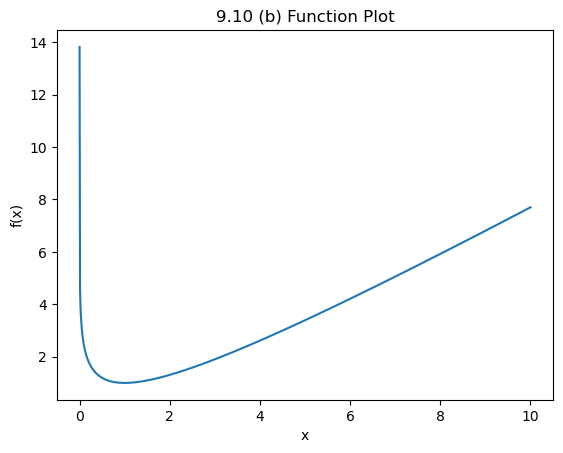
\includegraphics[width=0.7\textwidth]{HW5-9-10(b).png}
        \caption{Plot of $f(x)$}
    \end{figure}  

\begin{figure}[h!]
        \centering
        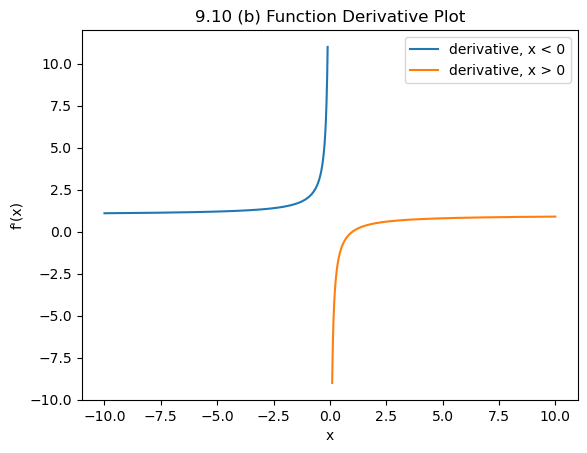
\includegraphics[width=0.7\textwidth]{HW5-9-10(b)-Derivative.png}
        \caption{Plot of $f^{'}(x)$}
    \end{figure}  
    
    \end{solution}
    
\end{enumerate}

Plot $f$ and $f^{'}$, and show the first few iterates.
\end{problem}

\newpage 
\begin{problem} \textit{Gradient and Newton methods for composition functions.} Suppose $\phi: \mathbb{R} \rightarrow \mathbb{R}$ is increasing and convex, and $f: \mathbb{R}^n \rightarrow \mathbb{R}$ is convex, so $g(x) = \phi(f(x))$ is convex. (We assume that f and g are twice differentiable.) The problems of minimizing f and minimizing g are clearly equivalent. \newline 
Compare the gradient method and Newton’s method, applied to f and g. How are the
search directions related? How are the methods related if an exact line search is used?
Hint. Use the matrix inversion lemma

\begin{solution} Analysis of Gradient Descent and Newton's Method

\textbf{\underline{Gradient Descent:}} \newline 
    Based on the chain rule, we can see that $\nabla g(x) = \phi'(f(x)) \nabla f(x)$. We are given information that $\phi(x)$ is increasing and convex. Hence, $\phi'(f(x)) = k_1$ where $k_1$ is a positive constant. 
    
    It is clear to see that the $\nabla g(x)$ is a positive multiple of $\nabla f(x)$.  
    
    When we do exact line search, since our descent direction is the negative gradient, this is what we are doing:

    $\arg \min_{s \geq 0} (f(x - s\nabla f(x)))$ for the case of $f$ \newline 
    $\arg \min_{s \geq 0} (g(x - s\nabla g(x)))$ for the case of $g$ \newline 

    We can basically see that the goal of Exact Line Search is to choose values of $s$ such that $f$ is minimized along the ray $-\nabla f(x)$ and $g$ is minimized along the ray $-\nabla g(x)$

    Let $s = s_1$ be the solution to $\arg \min_{s} (f(x - s\nabla f(x)))$


    We can express $\arg \min_{s} (g(x - s\nabla g(x)))$ as follows: \newline 
    $\arg \min_{s \geq 0} \phi((f(x - s\nabla g(x))))$ 

    $\arg \min_{s \geq 0} \phi((f(x - sk_1 \nabla f(x))))$

    Since $\phi(f(x))$ is convex and we know that convex functions are convex along any line, we can say that $\phi((f(x - sk_1 \nabla f(x))))$ is Convex. Hence, we can take the derivative, with respect to s, and set it to 0

    $\frac{d}{ds} (\phi((f(x - sk_1 \nabla f(x))))) = \phi'((f(x - sk_1 \nabla f(x)))) \frac{d}{ds} ((f(x - sk_1 \nabla f(x)))) = 0$

    Since convex functions are convex along any line, we know that $(f(x - s\nabla f(x)))$ is convex. Hence, at $s = s_1$, $\frac{d}{ds}(f(x - s\nabla f(x))) = 0$ \newline 

    Let's revisit $\phi'((f(x - sk_1 \nabla f(x)))) \frac{d}{ds} ((f(x - sk_1 \nabla f(x))))$. If we set $s = \frac{s_1}{k_1}$, we can see that $\frac{d}{ds} ((f(x - sk_1 \nabla f(x)))) = 0$ . This, by consequence, would means that $\phi'((f(x - sk_1 \nabla f(x)))) \frac{d}{ds} ((f(x - sk_1 \nabla f(x)))) = 0$ and we have minimized $(g(x - s\nabla g(x)))$

    Now let's calculate the next iterates. \newline 
    Let $x^+$ represent the next iterate

    For f, $x^+ = x - s_1 \nabla f(x)$

    FOr g, $x^+ = x - \frac{s_1}{k_1} \nabla g(x)$. This can be simplified to $x^+ = x - \frac{s_1}{k_1} k_1 \nabla f(x)$, $x^+ = x - s_1 \nabla f(x)$

    Hence, if we use exact line search, assuming we have the same starting iterate both gradient descent algorithms, the iterates of both gradient descent algorithms will be the same. However, if we use another method such as backtracking search, it may not be the same. 

\textbf{\underline{Newton's Method:}} \newline 
Based on the chain rule, $\nabla^2g(x) = \phi^{''}(f(x)) \nabla f(x) \nabla f(x)^T + \phi^{'}(f(x))\nabla^2f(x)$

Search Direction when Newton's Method is applied to $f$: $\Delta x_{nt} = -\nabla^2f(x)^{-1} \nabla f(x)$

Search Direction when Newton's Method is applied to $g$: $\Delta x_{nt} = -\nabla^2g(x)^{-1} \nabla g(x) = -(\phi^{''}(f(x)) \nabla f(x) \nabla f(x)^T + \phi^{'}(f(x))\nabla^2f(x))^{-1} ( \phi'(f(x)) \nabla f(x))$


According to the Matrix Inversion Lemma, we know that $(A + BC)^{-1} = A^{-1} - A^{-1}B (I + CA^{-1}B)^{-1} CA^{-1}$ \newline 

Let's work with $\Delta x_{nt}$ for $g$ 

We see that $\Delta x_{nt} = -(\phi^{''}(f(x)) \nabla f(x) \nabla f(x)^T + \phi^{'}(f(x))\nabla^2f(x))^{-1} ( \phi'(f(x)) \nabla f(x))$ \newline 

Let's define the following variables: 

$A = \phi^{'}(f(x))\nabla^2f(x)$ \newline 
$B = \phi^{''}(f(x))  \nabla f(x)$ \newline 
$C = \nabla f(x)^T$

Let's simplify $(\phi^{''}(f(x)) \nabla f(x) \nabla f(x)^T + \phi^{'}(f(x))\nabla^2f(x))^{-1}$ \newline 

Note: If $\phi^{''}(f(x)) = 0$, then the above simplifies to $(\phi^{'}(f(x))\nabla^2f(x))^{-1}$. This would mean that $x_{nt} = - (\phi^{'}(f(x))\nabla^2f(x))^{-1} ( \phi'(f(x)) \nabla f(x)) = -\nabla^2f(x)^{-1} \nabla f(x)$ which matches the Search Direction when Newton's Method is applied to $f$.

Since $\phi(x)$ is a convex function, $\phi^{''}(f(x)) \geq 0$. We have already proved what happens when $\phi^{''}(f(x)) = 0$. For the rest of the analysis, to address the case where $\phi^{''}(f(x)) > 0$, we will say that $\phi^{''}(f(x)) > 0$.

We know that $(A + BC)^{-1}$ can be expressed as: \newline 
$A^{-1} - A^{-1}B (I + CA^{-1}B)^{-1} CA^{-1}$ \newline 
Since we know that $C = \frac{1}{\phi^{''}(f(x))} B^T$, we can further simplify \newline

$A^{-1} - A^{-1}B (I + \frac{1}{\phi^{''}(f(x))} B^TA^{-1}B)^{-1} \frac{1}{\phi^{''}(f(x))} B^TA^{-1}$ \newline 
We know that $B$ is a column vector. We also know that $\phi^{'}(f(x))$ is positive and $\nabla^2f(x)$ is positive definite. Hence, $A$ is positive definite. Furthermore, since $\phi(x)$ is a convex function, $\phi^{''}(f(x)) \geq 0$. This means that $\frac{1}{\phi^{''}(f(x))} B^TA^{-1}B$ is a positive scalar number. Subsequently, $(I + \frac{1}{\phi^{''}(f(x))} B^TA^{-1}B)^{-1}$ is a positive scalar number as well. Hence, we can represent this positive scalar number as $k_1$. We can see that $k_1 < 1$

$(I + \frac{1}{\phi^{''}(f(x))} B^TA^{-1}B)^{-1} = k_1$

$A^{-1} - k_1 A^{-1}B \frac{1}{\phi^{''}(f(x))} B^TA^{-1}$ \newline 
$A^{-1} - \frac{k_1}{\phi^{''}(f(x))} A^{-1}B  B^TA^{-1}$ \newline 

$x_{nt} = -(A^{-1} - \frac{k_1}{\phi^{''}(f(x))} A^{-1}B  B^TA^{-1}) ( \phi'(f(x)) \nabla f(x))$

$x_{nt} = -(A^{-1} - \frac{k_1}{\phi^{''}(f(x))} A^{-1}B  B^TA^{-1}) ( \frac{\phi^{'}(f(x))}{\phi^{''}(f(x))} B)$

$x_{nt} = -(\frac{\phi^{'}(f(x))}{\phi^{''}(f(x))} A^{-1}B - \frac{k_1 \phi^{'}(f(x))}{(\phi^{''}(f(x)))^2} A^{-1}B  B^TA^{-1}B)$

Since $A$ is positive definite, $B^TA^{-1}B = k_2$ where $k_2$ is a positive constant

$x_{nt} = -(\frac{\phi^{'}(f(x))}{\phi^{''}(f(x))} A^{-1}B - \frac{k_1 k_2 \phi^{'}(f(x))}{(\phi^{''}(f(x)))^2} A^{-1}B)$

$x_{nt} = -( (\frac{\phi^{'}(f(x))}{\phi^{''}(f(x))} - \frac{k_1 k_2 \phi^{'}(f(x))}{(\phi^{''}(f(x)))^2}) (A^{-1}B))$

$x_{nt} = -((\frac{\phi^{'}(f(x))}{\phi^{''}(f(x))} - \frac{k_1 k_2 \phi^{'}(f(x))}{(\phi^{''}(f(x)))^2}) (\frac{\phi^{''}(f(x))}{\phi^{'}(f(x))} \nabla^2f(x)^{-1} \nabla f(x)))$


$x_{nt} = -(\nabla^2f(x)^{-1} \nabla f(x) ( 1 - \frac{k_1 k_2}{\phi^{''}(f(x))}))$

$x_{nt} = -\nabla^2f(x)^{-1} \nabla f(x) (1 - \frac{k_1 k_2}{\phi^{''}(f(x))})$

Let $k_3 = \frac{k_2}{\phi^{''}(f(x))}$. We see that $k_1 = (1 + k_3)^{-1}$. Hence, $k_1k_3 < 1$. This means that $x_{nt}$, when Newton's method is applied on $g$, is a positive multiple of $x_{nt}$, when Newton's method is applied on $f$.

Through our analysis, we can see that $x_{nt}$, when Newton's method is applied on $g$, is always a positive multiple of $x_{nt}$, when Newton's method is applied on $f$.

Based on our previous analysis when we were looking at Gradient Descent, our proof showed that, when the search directions are positive multiples of each other and when we are using EXACT LINE SEARCH, the iterates of the descent algorithms should be identical. 

This indicates to us that, when we perform exact line search with Newton's Method, the iterates should be the same for both $f$ and $g$. 

However, please keep in mind that this behavior is NOT guaranteed when we do backtracking line search. 


\end{solution}
\end{problem}


\end{document}





